\chapter{Final Mega Project: School Management System}

\section{Introduction: Real-Life Problem}

Every school must manage:
\begin{itemize}
    \item Student information
    \item Teacher details
    \item Marks and attendance
\end{itemize}

If everything is written on paper:
\begin{itemize}
    \item Data can be lost
    \item Searching is slow
    \item Mistakes are common
\end{itemize}

So schools use \textbf{School Management Software}.

In this chapter, we will build a \textbf{simple school management system} using Python.

\section{What Will We Use in This Project?}

This project combines everything students have learned.

\begin{center}
\begin{tabular}{|l|l|}
\hline
\textbf{Concept} & \textbf{Usage} \\
\hline
Variables & Store data \\
Functions & Perform tasks \\
OOP & Student and Teacher classes \\
File Handling & Save data \\
Error Handling & Prevent crashes \\
Modules & Organize code \\
Tkinter & Build GUI \\
\hline
\end{tabular}
\end{center}

\section{System Features}

Our system will:
\begin{itemize}
    \item Add student records
    \item Display saved students
    \item Save data permanently
    \item Use a simple GUI
\end{itemize}

\section{Step 1: Design the System}

\subsection{Real-Life Design Thinking}

Think like a school:
\begin{itemize}
    \item Each student has name and roll
    \item Data must be saved
    \item User clicks buttons
\end{itemize}

\section{Step 2: Student Class (OOP)}

\begin{verbatim}
class Student:
    def __init__(self, name, roll):
        self.name = name
        self.roll = roll

    def to_string(self):
        return self.name + "," + self.roll
\end{verbatim}

\section{Step 3: File Handling Module}

\begin{verbatim}
def save_student(student):
    with open("students.txt", "a") as file:
        file.write(student.to_string() + "\n")

def load_students():
    with open("students.txt", "r") as file:
        return file.readlines()
\end{verbatim}

\section{Step 4: GUI Design (Tkinter)}

\begin{verbatim}
import tkinter as tk
from student import Student
from storage import save_student, load_students

def add_student():
    try:
        name = entry_name.get()
        roll = entry_roll.get()
        student = Student(name, roll)
        save_student(student)
        label_status.config(text="Student saved")
    except:
        label_status.config(text="Error saving student")

window = tk.Tk()
window.title("School Management System")

entry_name = tk.Entry(window)
entry_name.pack()
entry_name.insert(0, "Student Name")

entry_roll = tk.Entry(window)
entry_roll.pack()
entry_roll.insert(0, "Roll Number")

btn_add = tk.Button(window, text="Add Student", command=add_student)
btn_add.pack()

label_status = tk.Label(window, text="")
label_status.pack()

window.mainloop()
\end{verbatim}

\section{Step 5: Displaying Saved Students}

\begin{verbatim}
def show_students():
    students = load_students()
    text_box.delete("1.0", tk.END)
    for s in students:
        text_box.insert(tk.END, s)

btn_show = tk.Button(window, text="Show Students", command=show_students)
btn_show.pack()

text_box = tk.Text(window, height=10)
text_box.pack()
\end{verbatim}

\section{Diagram: System Architecture}

\begin{center}
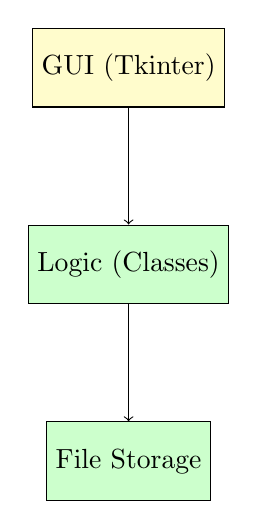
\begin{tikzpicture}[node distance=2.5cm]
\node (gui) [draw, rectangle, fill=yellow!20, minimum height=1cm] {GUI (Tkinter)};
\node (logic) [draw, rectangle, fill=green!20, below of=gui, minimum height=1cm] {Logic (Classes)};
\node (file) [draw, rectangle, fill=green!20, below of=logic, minimum height=1cm] {File Storage};

\draw[->] (gui) -- (logic);
\draw[->] (logic) -- (file);
\end{tikzpicture}
\end{center}

\section{How This Project Helps Students}

Students learn:
\begin{itemize}
    \item How real software is designed
    \item How different concepts work together
    \item Confidence to build applications
\end{itemize}

\section{Possible Improvements (For Students)}

\begin{itemize}
    \item Add teacher records
    \item Add marks and attendance
    \item Add login system
    \item Improve GUI design
\end{itemize}

\section{Key Concepts Used}

\begin{itemize}
    \item OOP for data modeling
    \item File handling for memory
    \item GUI for user interaction
    \item Error handling for safety
\end{itemize}

\section{End-of-Chapter Exercises}

\subsection{Project-Based Questions}

\begin{enumerate}
    \item Add student age field.
    \item Add delete student option.
    \item Save data in different files.
\end{enumerate}

\subsection{Thinking Questions}

\begin{enumerate}
    \item Why is this project useful in real life?
    \item Which part was most difficult?
    \item How can this system be improved?
\end{enumerate}

\section{Teacher Notes}

\marginnote{
\textbf{Learning Objectives}
\begin{itemize}
    \item Students integrate all concepts
    \item Students build complete software
    \item Students develop problem-solving skills
\end{itemize}

\textbf{Teaching Tips}
\begin{itemize}
    \item Encourage teamwork
    \item Demonstrate step-by-step building
    \item Allow creativity
\end{itemize}

\textbf{Assessment}
\begin{itemize}
    \item Working program
    \item Correct use of concepts
    \item Code clarity
\end{itemize}
}